\documentclass[12pt]{article}
\usepackage[LGR, T1]{fontenc}
\usepackage[utf8]{inputenc}
\usepackage[greek,english]{babel}
\usepackage{alphabeta}
\usepackage{multicol}
\usepackage[margin=0.8in]{geometry}
\usepackage{microtype}
\usepackage{csvsimple}
\usepackage{multirow}
\usepackage{graphicx}
\usepackage{tikz}
\usepackage{hyperref}
\usepackage{algorithm} 
\usepackage{algorithmic}
\usepackage{csquotes}
\usepackage{amsmath}
\usepackage{amssymb}
\usepackage{alphabeta}
\usepackage{pgfgantt}
\usepackage{xcolor}  
\usepackage{framed}
\usepackage{listings}
\usepackage{tabularx}
\usepackage{adjustbox}
\usepackage{caption}
\usepackage{minted}
\usepackage{cite}
\usepackage{textcomp}
\usepackage{subfigure}
\usepackage{subcaption}



\title{Εργαστηριακή Άσκηση 2 \\ Βασικοί Γεωμετρικοί Μετασχηματισμοί}
\author{Μαριάνθη Θώδη}
\date{Νοέμβριος 2025}

\begin{document}
\begin{figure}
\begin{flushleft}
  
\includegraphics[width=6cm]{logo.png}
  \hfill
\end{flushleft}
\end{figure}

\maketitle
\newpage
\tableofcontents

\section{Abstract}
Η παρούσα εργαστηριακή άσκηση έχει ως στόχο την εξοικείωση με τους γεωμετρικούς μετασχηματισμούς και την εφαρμογή τους στη δημιουργία κινούμενων εικόνων χρησιμοποιώντας το matlab. Αρχικά, παρουσιάζεται η χρήση βασικών συναρτήσεων
με σύντομη περιγραφή της λειτουργίας κάθε μίας. Στη συνέχεια, εφαρμόζονται μετασχηματισμοί κλιμάκωσης για τη σύνθεση σύνθετων εικόνων και μετασχηματισμοί στρέβλωσης για τη δημιουργία περιοδικών ακολουθιών βίντεο. Επιπλέον, υλοποιούνται μετασχηματισμοί περιστροφής, κλιμάκωσης και μετατόπισης για την παραγωγή βίντεο με κινούμενα αντικείμενα, με χρήση μάσκας. Η άσκηση ολοκληρώνεται με πειραματισμό διαφορετικών μεθόδων παρεμβολής,
καταγραφή της ποιότητας των αποτελεσμάτων και τροποποίηση των μετασχηματισμών για την προσαρμογή της πορείας των αντικειμένων.
Ο πλήρης κώδικας και τα παραδείγματα της άσκησης διατίθενται σε repo στο GitHub στον αντίστοιχο σύνδεσμο \href{https://github.com/palpatinedude/Computer-Vision-.git}{GitHub Repository}.

\section{Εξοικείωση με Βασικές Συναρτήσεις}
\begin{table}[h!]
    \centering
    \begin{tabular}{|l|p{10cm}|}
    \hline
    \textbf{Συνάρτηση MATLAB} & \textbf{Επεξήγηση} \\
    \hline
    imread & Φορτώνει μία εικόνα από αρχείο στον χώρο εργασίας του matlab ως πίνακα . \\
    \hline
    imwarp & Εφαρμόζει γεωμετρικό μετασχηματισμό (affine ή projective) σε εικόνα.\\
    \hline
    affine2d & Δημιουργεί αντικείμενο affine μετασχηματισμού (κλιμάκωση, περιστροφή, διάτμηση) ,απαιτεί μητρώο 3x3. \\
    \hline
    projective2d & Δημιουργεί projective μετασχηματισμό, χρησιμοποιείται για παραμορφώσεις όπως προοπτικές προβολές. \\
    \hline
    imref2d &Καθορίζει το μέγεθος και το σύστημα αναφοράς της εξόδου. \\
    \hline
    implay & Αναπαράγει ακολουθία εικόνων ως βίντεο. \\
    \hline
    \end{tabular}
    \caption{Συνήθεις συναρτήσεις MATLAB για επεξεργασία εικόνας και βίντεο}
    \end{table}


\section{Κλιμάκωση Εικόνας}
Για την υλοποίηση του ερωτήματος 2 χρησιμοποιήθηκε affine μετασχηματισμός κλιμάκωσης μέσω της συνάρτησης affine2d. Δημιουργήθηκαν πολλαπλές εκδόσεις της ίδιας εικόνας ball.jpg με διαφορετικούς συντελεστές κλιμάκωσης,
οι οποίες κεντραρίστηκαν σε καμβά ίδιου μεγέθους και στη συνέχεια συντέθηκαν σε μία ενιαία εικόνα - scaledversions.png.
\newpage
\begin{figure}[h!]
    \begin{center}
    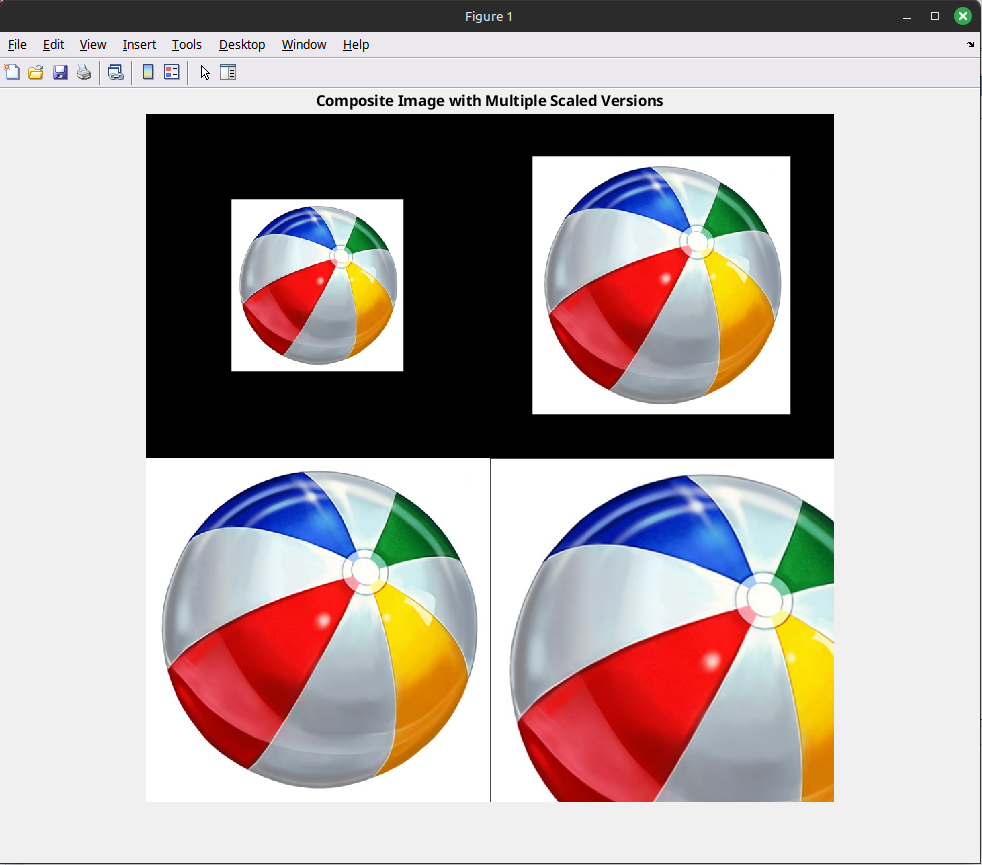
\includegraphics[width=7cm]{scaledversions.png}
    \caption{Multiple scaled versions of the same image}
    \label{fig:drlagent}
    \end{center}
    \end{figure}
    

\section{Δημιουργία Βίντεο με Shearing Εικόνας}
Στην άσκηση αυτή, εφαρμόστηκε horizontal shear στην εικόνα \texttt{pudding.png} για τη δημιουργία μιας περιοδικής ακολουθίας εικόνων. 
Η μεταβολή της τιμής της στρέβλωσης ακολουθεί ημιτονοειδή μορφή, ώστε να επιτυγχάνεται περιοδικότητα της κίνησης και κάθε καρέ της ακολουθίας δημιουργήθηκε με τη χρήση affine μετασχηματισμού και της συνάρτησης \texttt{imwarp}, ενώ διατηρήθηκαν οι διαστάσεις της αρχικής εικόνας μέσω του \texttt{imref2d}. Τέλος, η ακολουθία των καρέ αποθηκεύτηκε σε βίντεο με το όνομα \texttt{sheared\_pudding.avi}.
    

\section{Περιοδική Οριζόντια Διάτμηση με Σταθερή Βάση}
Στην άσκηση αυτή εφαρμόστηκε οριζόντια διάτμηση στην εικόνα \texttt{pudding.png}, διατηρώντας όμως σταθερή τη βάση της εικόνας. Κάθε καρέ της ακολουθίας μετατοπίζεται κατάλληλα ώστε το κάτω μέρος της εικόνας να παραμένει στη θέση του, όπου ο υπολογισμός της μετατόπισης γίνεται ως εξής:
    
\[
\text{translateX} = - \text{shearX} \cdot (H - 1)
\]
    
όπου \( H \) είναι το ύψος της εικόνας. Με αυτόν τον τρόπο, η βάση της εικόνας δεν μετακινείται καθώς τα πάνω τμήματα της εικόνας στρεβλώνονται.
Η μεταβολή της τιμής της στρέβλωσης ακολουθεί ημιτονοειδή μορφή για περιοδικότητα της κίνησης, και η ακολουθία των καρέ αποθηκεύτηκε σε βίντεο με το όνομα \texttt{sheared\_pudding.avi}.
    

\section{Ανεμόμυλος με μάσκα}
Στόχος του ερωτήματος αυτού είναι ,η δημιουργία animation όπου περιστρέφονται οι λεπίδες του ανεμόμυλου πάνω σε φόντο, με τη βάση τους σταθερή και χωρίς να εμφανίζονται μαύρες γραμμές περιμετρικά.
\subsection{Λογική}
Ο τρόπος τοποθέτησης των blades πάνω στο φόντο ξεκινά με τη φόρτωση των εικόνων που θα χρησιμοποιηθούν στο animation: το φόντο (\texttt{windmill\_back.jpeg}), οι λεπίδες (\texttt{windmill.png}) και η αντίστοιχη μάσκα τους (\texttt{windmill\_mask.png}). Η μάσκα καθορίζει ποια pixels ανήκουν στις λεπίδες και ποια όχι, επιτρέποντας την επιλεκτική επικόλληση στο background. 
Στη συνέχεια υπολογίζεται η ακριβής θέση των blades έτσι ώστε η βάση τους να παραμένει σταθερή κατά την περιστροφή, ενώ απομονώνεται ένα patch του φόντου (\texttt{bgPatch}) ίδιου μεγέθους με τις λεπίδες. Το patch αυτό χρησιμοποιείται για να αντικαταστήσει τα μαύρα pixels που μπορεί να εμφανιστούν κατά την περιστροφή, διατηρώντας την εικόνα ομοιογενή και χωρίς ανεπιθύμητες μαύρες άκρες. \\
Τώρα η περιστροφή των λεπίδων γίνεται με τη συνάρτηση \texttt{imrotate}, χρησιμοποιώντας την επιλογή \texttt{"nearest"} interpolation ώστε οι τιμές των pixels να μην αλλοιώνονται από μέσους όρους (αποφεύγονται σκοτεινές άκρες) και την επιλογή \texttt{"crop"} ώστε το μέγεθος να παραμένει ίδιο με το αρχικό. 
Μετά την περιστροφή, τα pixels που γίνονται εντελώς μαύρα αντικαθίστανται με τα αντίστοιχα από το \texttt{bgPatch}, εξαλείφοντας τυχόν μαύρες γραμμές γύρω από τις λεπίδες. Τέλος, εφαρμόζεται η μάσκα ώστε μόνο τα pixels των blades να ενημερώνουν το background, διατηρώντας αναλλοίωτα τα υπόλοιπα pixels και εξασφαλίζοντας ένα ομαλό αποτέλεσμα στο τελικό animation (\texttt{transf\_windmill\_fixed\_base.avi}).

\section{Παράμετροι παρεμβολής}

\section{Κίνηση μπάλας στην παραλία}




\end{document}